\begin{figure}[h!]
\centering
\pgfkeys{/pgf/number format/.cd,1000 sep={}}
\pgfplotsset{every axis legend/.style={
cells={anchor=center},% Centered entries
inner xsep=3pt,inner ysep=2pt,nodes={inner sep=2pt,text depth=0.15em},
anchor=north west,
shape=rectangle,
fill=none,
%draw=none,
%at={(rel axis cs:0.04,0.88)}
at={(rel axis cs:0.4,0.3)}
}
}
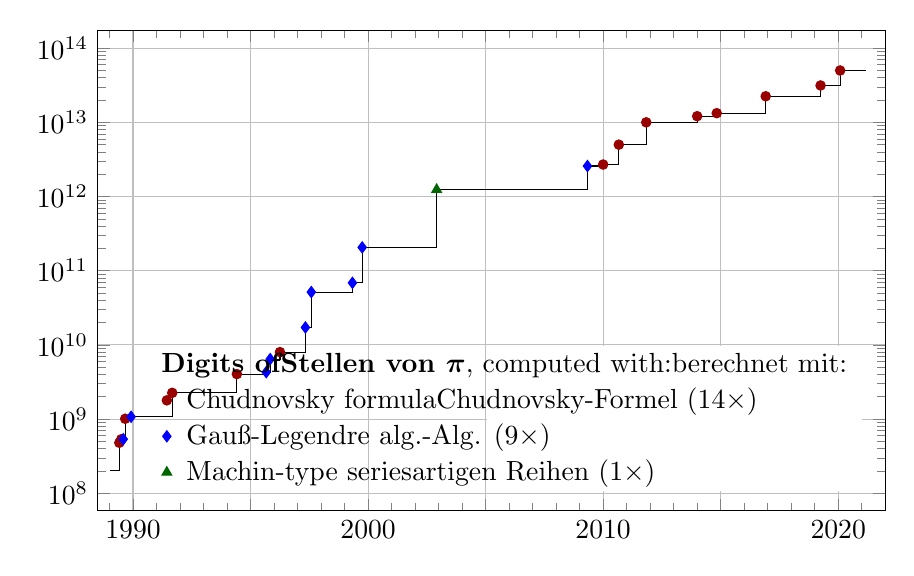
\begin{tikzpicture}
\begin{semilogyaxis}[scale only axis=true,
  width=10cm, height=6.1cm,
  %width=9.2cm, height=\en{3.65cm}\de{3.35cm},
  legend cell align={left},
  minor x tick num=4,
  %xtick={1990,2000,2010,2020},
  %minor tick length = 6pt,
 % xtick={1990,1991,2000,2001,2010,2011,2020,2021},
  %xtick={1990,2000,2010,2020},
  minor xtick={1989,1991,1992,1993,1994,1995,1996,1997,1998,1999,
                    2001,2002,2003,2004,2005,2006,2007,2008,2009,
                    2011,2012,2013,2014,2015,2016,2017,2018,2019,2021},
  xticklabels={,,1990,,2000,,2010,,2020,},
  grid=major, 
    major grid style=gray!50,
  ytick={1e8,1e9,1e10,1e11,1e12,1e13,1e14},
  xmin=1988.5,
  xmax=2022,
  yticklabel pos=left,
  %x tick label as interval,
  %ylabel=\en{decimal digits of}\de{Dezimalen von} $\pi$,
legend pos = south east]%,xlabel=\en{year}\de{Jahr}]
\addlegendimage{empty legend}\addlegendentry{\hspace{-.2cm}\textbf{\en{Digits of}\de{Stellen von} \boldmath{$\pi$}}, \en{computed with:}\de{berechnet mit:}}
%\addplot[only marks, mark size=0pt] coordinates { (1999.666667, 1011196691) };
%\addplot[only marks, mark size=0pt] coordinates { (1999.666667, 1011196691) };
%\addplot[only marks, mark size=0pt] coordinates { (1999.666667, 1011196691) };
\addplot[only marks, mark=*, mark size=1.7pt, red!60!black] coordinates {
(1989.416667, 480000000) % Chudnovsky brothers (Chud)
(1989.500000, 535339270) % Chudnovsky brothers (Chud)
(1989.666667, 1011196691) % Chudnovsky brothers (Chud)
(1991.666667, 2260000000) % Chudnovsky brothers (Chud)
(1994.416667, 4044000000) % Chudnovsky brothers (Chud)
(1996.250000, 8000000000) % Chudnovsky brothers (Chud)
(2010.000000, 2699999990000) % Fabrice Bellard (Chud)
(2010.666667, 5000000000000) % Shigeru Kondo & Alex Yee (Chud)
(2011.833333, 10000000000050) % Shigeru Kondo (Chud)
(2014.000000, 12100000000050) % Shigeru Kondo (Chud)
(2014.833333, 13300000000000) % Sandon van Ness (Chud)
(2016.916667, 22459157718361) % Peter Trueb (Chud)
(2019.250000, 31415926535897) % Emma Haruka Iwao (Chud)
(2020.083333, 50000000000000) % Timothy Mullican (Chud)
};
%\draw [fill=black,black] (1990,2e7) rectangle (1991,10e7);
%\draw [fill=black,black] (1990,10e13) rectangle (1991,2e14);
%\draw [fill=black,black] (2000,2e7) rectangle (2001,10e7);
%\draw [fill=black,black] (2000,10e13) rectangle (2001,2e14);
%\draw [fill=black,black] (2010,2e7) rectangle (2011,10e7);
%\draw [fill=black,black] (2010,10e13) rectangle (2011,2e14);
%\draw [fill=black,black] (2020,2e7) rectangle (2021,10e7);
%\draw [fill=black,black] (2020,10e13) rectangle (2021,2e14);
\draw [fill=white,white] (2005.1,1.1e8) rectangle (2021,0.95e10);
\addplot[only marks, mark=diamond*, blue] coordinates { 
%(1982, 2097144) % GL2
%(1982, 4194288) % GL2
%(1982, 8388576) % GL2
%(1983, 16777206) % GL2
%(1986.083333, 29360111) % B2. B4
%(1986.75, 33554414) % GL2. B4
%(1986.833333, 67108839) % GL2
%(1987.083333, 134214700) % GL2. B4
%(1988.083333, 201326551) % Kanada et al (GL2, B4)
(1989.583333, 536870898) % Kanada et al (GL2, B4)
(1989.916667, 1073740799) % Kanada et al (GL2)
(1995.666667, 4294960000) % Kanada et al (GL2, B4)
(1995.833333, 6442450000) % Kanada et al (GL2, B4)
(1997.333333, 17179869142) % Kanada et al (GL2, B4)
(1997.583333, 51539600000) % Kanada et al (GL2, B4)
(1999.333333, 68719470000) % Kanada et al (GL2, B4)
(1999.750000, 206158430000) % Kanada et al (GL2, B4)
(2009.333333, 2576980377524) % Daisuke et al (GL2, B4)
};

\addplot[only marks, mark=triangle*, green!40!black] coordinates {
%(1981, 2000036) % arctan
%(1981, 2000050) % ?
(2002.916667, 1241100000000) % Kanada et al (Machin-Type)
};
%\addplot[dotted]  coordinates { (1988.083333, 201326551)(1989.0, 201326551)};
\addplot[solid]  coordinates { 
%(1988.083333, 201326551)
(1989.0, 201326551)
(1989.416667, 201326551) 
(1989.416667, 480000000) 
(1989.500000, 480000000) 
(1989.500000, 535339270) 
(1989.583333, 535339270) 
(1989.583333, 536870898) 
(1989.666667, 536870898) 
(1989.666667, 1011196691)
(1989.916667, 1011196691) 
(1989.916667, 1073740799) 
(1991.666667, 1073740799)
(1991.666667, 2260000000) 
(1994.416667, 2260000000)
(1994.416667, 4044000000) 
(1995.666667, 4044000000)
(1995.666667, 4294960000) 
(1995.833333, 4294960000)
(1995.833333, 6442450000) 
(1996.250000, 6442450000) 
(1996.250000, 8000000000) 
(1997.333333, 8000000000)
(1997.333333, 17179869142)
(1997.583333, 17179869142)
(1997.583333, 51539600000) 
(1999.333333, 51539600000) 
(1999.333333, 68719470000) 
(1999.750000, 68719470000) 
(1999.750000, 206158430000) 
(2002.916667, 206158430000) 
(2002.916667, 1241100000000) 
(2009.333333, 1241100000000)
(2009.333333, 2576980377524) 
(2010.000000, 2576980377524) 
(2010.000000, 2699999990000) 
(2010.666667, 2699999990000) 
(2010.666667, 5000000000000) 
(2011.833333, 5000000000000) 
(2011.833333, 10000000000050)
(2014.000000, 10000000000050) 
(2014.00000, 12100000000050) 
(2014.833333, 12100000000050)
(2014.833333, 13300000000000)
(2016.916667, 13300000000000) 
(2016.916667, 22459157718361) 
(2019.250000, 22459157718361)
(2019.250000, 31415926535897)
(2020.083333, 31415926535897)
(2020.083333, 50000000000000) 
(2021.2, 50000000000000) }; 

%\addplot[only marks, mark=pentagon*, orange!40!black] coordinates {
%(1985.833333, 17526200) % Rama
%};

\addlegendentry{~\en{Chudnovsky formula}\de{Chudnovsky-Formel} (14$\small{\times}$)};
\addlegendentry{~Gauß-Legendre\en{ alg.}\de{-Alg.} (9$\small{\times}$)};
\addlegendentry{~Machin-\en{type series}\de{artigen Reihen} (1$\small{\times}$)};
%\addlegendentry{~\en{Ramanujan's formula}\de{Ramanujan-Formel} (1)}
\end{semilogyaxis}
\end{tikzpicture}\vspace*{-8pt}
\caption{\en{Number of known digits of $\pi$ since 1989}\de{Anzahl bekannter Stellen von $\pi$ seit 1989}}
\label{\en{EN}fighist}
\end{figure}